\subsection{Distributed Pose Graph Optimization}
In distributed PGO \cite{tron2014distributed,choudhary2017distributed,tian2019distributed}, we are given $|\AA|$ nodes $\AA\triangleq\{1,\,2,\,\cdots,\, |\AA|\}$ and each node $\alpha\in\AA$ has $n_\alpha$ poses $g_{1}^\alpha$, $g_{2}^\alpha$, $\cdots$, $g_{n_\alpha}^\alpha\in SE(d)$. Let $g_{(\cdot)}^\alpha\triangleq(t_{(\cdot)}^\alpha,\,R_{(\cdot)}^\alpha)$ where $t_{(\cdot)}^\alpha\in\R^d$ is the translation and $R_{(\cdot)}^\alpha\in SO(d)$ the rotation.  We consider the problem of estimating unknown poses $g_{1}^\alpha$, $g_{2}^\alpha$, $\cdots$, $g_{n_\alpha}^\alpha\in SE(d)$ for all the nodes $\alpha\in\AA$ given intra-node noisy measurements $\tilde{g}_{ij}^{\alpha\alpha}\triangleq(\nt_{ij}^{\alpha\alpha},\,\nR_{ij}^{\alpha\alpha})\in SE(d)$ of the relative pose
\vspace{-0.25em}
\begin{equation}\label{eq::gijaa}
g_{ij}^{\alpha\alpha} \triangleq \big({g_i^\alpha}\big)^{-1} g_j^\alpha\in SE(d)
\end{equation}
within a single node $\alpha$, and inter-node noisy measurements $\tilde{g}_{ij}^{\alpha\beta}\triangleq(\nt_{ij}^{\alpha\beta},\,\nR_{ij}^{\alpha\beta})\in SE(d)$ of the relative pose
\begin{equation}\label{eq::gijab}
g_{ij}^{\alpha\beta} \triangleq \big({g_i^\alpha}\big)^{-1} g_j^\beta\in SE(d)
\end{equation}
between different nodes $\alpha\neq\beta$.  In \cref{eq::gijaa,eq::gijab}, note that $\nt_{ij}^{\alpha\alpha}$ and $\nt_{ij}^{\alpha\beta}\in\R^d$ are translational measurements, and $\nR_{ij}^{\alpha\alpha}$ and $\nR_{ij}^{\alpha\beta}\in SO(d)$ are rotational measurements.

%Following \cite{rosen2016se}, we model distributed PGO as a directed graph $\aGG\triangleq(\VV,\aEE)$ whose vertices are ordered pairs consisting of node index, e.g., $\alpha$ and $\beta$  and pose index, e.g., $i$ and $j$. In the directed graph $\aGG$, the vertex $(\alpha,\,i)\in\VV$ is in one-to-one correspondence with the unknown pose $g_i^\alpha\in SE(d)$ and the directed edge $((\alpha,\,i),\,(\beta,\,j))\in \aEE$ is in one-to-one correspondence with the noisy measurement $\tilde{g}_{ij}^{\ab}\in SE(d)$. Note that $\aEE^{\ab}$, $\NN_-^\alpha$, $\NN_+^\alpha$ and $\NN^\alpha$ in \cref{eq::aEE,eq::NN,eq::NN+,eq::NN-} are well defined for distributed PGO.

Following \cref{eq::aEE,eq::NN-,eq::NN+,eq::NN}, we represent distributed PGO as  a directed graph  $\aGG=(\VV,\,\aEE)$ such that  unknown pose $g_i^\alpha\in SE(d)$ and noisy measurement $\tilde{g}_{ij}^{\ab}\in SE(d)$ have one-to-one correspondence to vertex $(\alpha,\,i)\in\VV$   and  directed edge $((\alpha,\,i),\,(\beta,\,j))\in \aEE$, respectively.  We refer nodes $\alpha$ and $\beta\in\AA$ as neighbors as long as either $\aEE^{\ab}\neq\emptyset$ or $\aEE^{\ba}\neq\emptyset$. Then,  $\NN_-^\alpha$ and $\NN_+^\alpha$ are the sets of neighbors with a directed edge from and to node $\alpha$, respectively, and $\NN^\alpha$ is the set of neighbors with a directed edge connected to node $\alpha$.

In the rest of this paper, we make the following assumption that each node can communicate with its neighbors and the network topology is unchanged during optimization. These assumptions  are common in distributed PGO \cite{choudhary2017distributed,tian2019distributed,tron2014distributed,eric2020geod}.
\begin{assumption}\label{assumption::neighbor}
	Each node $\alpha$ can communicate with its neighbors $\beta\in\NN^\alpha$ and the network topology is fixed.
\end{assumption}
\vspace{-1.25em}

\subsection{Loss Kernels}
In practice, it is inevitable that there exist inter-node measurements that are outliers resulting from false loop closures. These outliers adversely affect the overall  performance of distributed PGO. To address this issue, it is popular to use non-trivial loss kernels---e.g., Huber and Welsch losses---to enhance the robustness of distributed PGO \cite{agarwal2013robust,carlone2018convex,barron2019cvpr}.

In this paper, we make the following assumption that applies to a broad class of loss kernels $\rho(\cdot):\R^+\rightarrow\R$ in robotics and computer vision.
\vspace{-0.25em}
\begin{assumption}\label{assumption::loss}
	The loss kernel $\rho(\cdot):\R^+\rightarrow\R$ satisfies the following properties:
	\begin{enumerate}[(a)]
		\item $\rho(s)\geq 0$ for any $s\in\R^+$ and the equality ``$=$'' holds if and only if $s=0$;
		\item $\rho(\cdot):\R^+\rightarrow\R$ is continuously differentiable;\label{assumption::loss_cont}
		\item $\rho(\cdot):\R^+\rightarrow \R$ is a concave function;\label{assumption::loss_mono}
		\item $0\leq\nabla\rho(s)\leq 1$ for any $s\in\R^+$ and $\nabla\rho(0)=1$;\label{assumption::loss_drho}
		\item $\varphi(\cdot):\R^{m\times n}\rightarrow \R$ with $\varphi(X)\triangleq\rho(\|X\|^2)$ has Lipschitz continuous gradient, i.e., there exists $\mu>0$ such that $\|\nabla\varphi(X)-\nabla\varphi(X')\|\leq \mu\cdot\|X-X'\|$ for any $X,\,X'\in\R^{m\times n}$. \label{assumption::loss_L}
	\end{enumerate}
\end{assumption}

In the following, we present some examples of loss kernels (see \cref{fig::robust_loss}) satisfying \cref{assumption::loss}.

\begin{example}[Trivial Loss]\label{example::trivial}
	\begin{equation}\label{eq::trivial}
		\rho(s) =s.
	\end{equation}
\end{example}
\begin{example}[Huber Loss]\label{example::huber}
	\begin{equation}\label{eq::huber}
		\rho(s) =\begin{cases}
			s, & |s|\leq a,\\
			2\sqrt{a|s|}-a, & |s|\geq a
		\end{cases}
	\end{equation}
	where $a>0$.
\end{example}
\begin{example}[Welsch Loss]\label{example::GM}
	\begin{equation}\label{eq::geman}
		\rho(s) = a - a\exp\left(-\frac{s}{a}\right)
	\end{equation}
	where $a>0$.
\end{example}

\begin{figure}
	\centering
	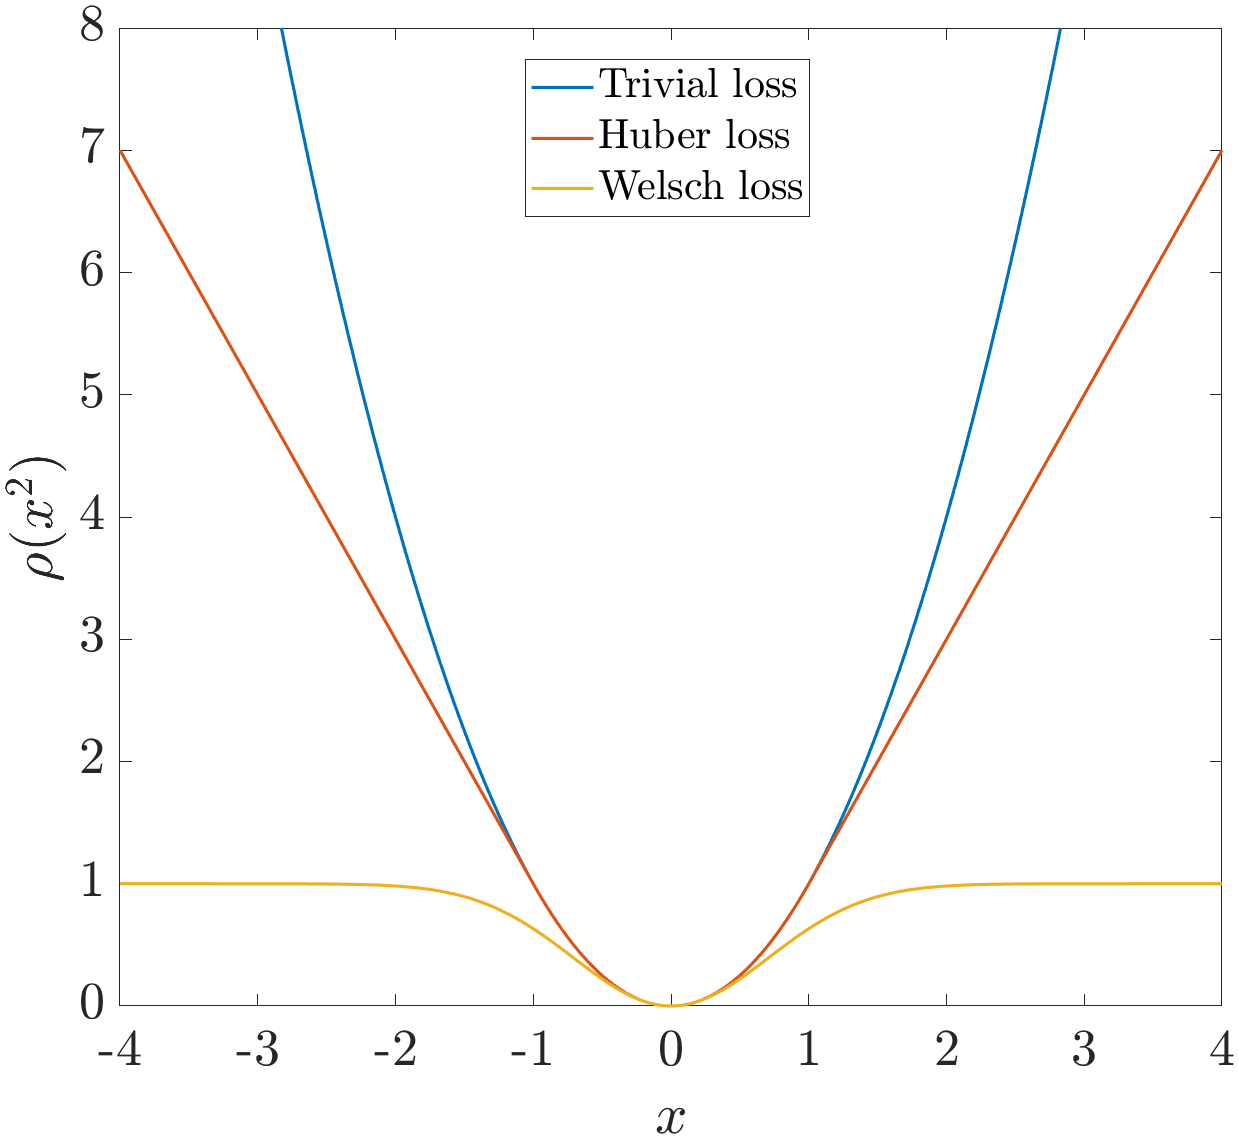
\includegraphics[width=0.3\textwidth]{figures/robust.png}
	\caption{$\rho(x^2)$ for the trivial, Huber, Welsch loss kernels.}\label{fig::robust_loss}
	\vspace{-1em}
\end{figure}

\vspace{-0.5em}
\subsection{Objective Function}
Recall that each node $\alpha\in\AA$ has $n_\alpha$ unknown poses $g_{1}^\alpha$, $g_{2}^\alpha$, $\cdots$, $g_{n_\alpha}^\alpha\in SE(d)$. For notational simplicity, we define $\XXa$ and $\XX$ as
\begin{equation}
\nonumber
\XXa\triangleq \R^{d\times n_\alpha}\times SO(d)^{n_\alpha}
\end{equation}
and
\begin{equation}
	\nonumber
	\XX \triangleq  \XX^1\times\cdots\times \XX^{|\AA|} \subset \R^{d\times (d+1)n},
\end{equation}
respectively, where $n\triangleq\sum_{\alpha\in\AA} n_\alpha$. Furthermore, we represent $g_i^\alpha\in SE(d)$, i.e., the $i$-th pose of node $\alpha\in\AA$, as a $d\times(d+1)$ matrix
\begin{equation}\label{eq::Xai}
	X_i^\alpha \triangleq \begin{bmatrix}
		t_i^\alpha & R_i^\alpha
	\end{bmatrix}\in SE(d)\subset \R^{d\times(d+1)},
\end{equation}
represent $(g_{1}^\alpha$, $g_{2}^\alpha$, $\cdots$, $g_{n_\alpha}^\alpha)\in SE(d)^{n_\alpha}$, i.e., all the poses of node $\alpha\in\AA$, as an element of $\XXa$ as well as a $d\times (d+1)n_\alpha$ matrix
\begin{equation}\label{eq::Xa}
	X^\alpha\triangleq \begin{bmatrix}
		t^\alpha & R^\alpha
	\end{bmatrix}\in \XXa \subset \R^{d\times (d+1)n_\alpha},
\end{equation}
where
$$
\vphantom{\Big\{}t^\alpha\triangleq\begin{bmatrix}
	t_1^\alpha & \cdots & t_{n_\alpha}^\alpha
\end{bmatrix}\in \R^{d\times n_\alpha}
$$
and
$$
R^\alpha\triangleq\begin{bmatrix}
	R_1^\alpha & \cdots & R_{n_\alpha}^\alpha
\end{bmatrix}\in SO(d)^{n_\alpha}\subset\R^{d\times dn_\alpha},
$$
and represent $\{(g_{1}^\alpha$, $g_{2}^\alpha$, $\cdots$, $g_{n_\alpha}^\alpha)\}_{\alpha\in\AA}\in SE(d)^{n}$, i.e., all the poses of distributed PGO, as an element of $\XX$ as well as a $d\times(d+1)n$ matrix
\begin{equation}\label{eq::Xall}
	X\triangleq\begin{bmatrix}
		X^1 & \cdots & X^{|\AA|}
	\end{bmatrix}\in \XX\subset \R^{d\times(d+1)n}.
\end{equation}

\begin{remark}
	$\XXa$ and $\XX$ are by definition homeomorphic to $SE(d)^{n_\alpha}$ and $SE(d)^n$, respectively. Thus, $\Xa\in\XXa$ and $X\in\XX$ are sufficient to represent elements of $SE(d)^{n_\alpha}$ and $SE(d)^n$.
\end{remark}

Following \cite{rosen2016se,fan2020mm,fan2019proximal}, distributed PGO can be formulated as an optimization problem on $X=\begin{bmatrix}
	X^1 & \cdots & X^{|\AA|}
\end{bmatrix}\in \XX$:
\begin{problem}[Distributed Pose Graph Optimization]
\begin{equation}\label{eq::pgo}
	\min_{X\in \XX} F(X).
\end{equation}
The objective function $F(X)$ in \cref{eq::pgo} is defined as
\begin{multline}\label{eq::obj}
F(X)\triangleq \sum_{\alpha\in\AA}\sum_{(i,j)\in \aEE^{\alpha\alpha}}\frac{1}{2}\Big[\kappa_{ij}^{\alpha\alpha}\|R_i^\alpha \nR_{ij}^{\alpha\alpha} -R_j^\alpha\|^2 +\\ \tau_{ij}^{\alpha\alpha}\|R_i^\alpha \nt_{ij}^{\alpha\alpha}+t_i^\alpha - t_j^\alpha\|^2\Big]+\\
\sum_{\substack{\alpha,\beta\in\AA,\\
		\alpha\neq \beta}}\sum_{(i,j)\in \aEE^{\alpha\beta}}\frac{1}{2}\Big[\rho\left(\kappa_{ij}^{\alpha\beta}\|R_i^\alpha \nR_{ij}^{\alpha\beta} -R_j^\beta\|^2\right. +\\ 
\left.\tau_{ij}^{\alpha\beta}\|R_i^\alpha \nt_{ij}^{\alpha\beta}+t_i^\alpha - t_j^\beta\|^2\right)\Big],
\end{multline}
where $\kappa_{ij}^{\alpha\alpha}$, $\tau_{ij}^{\alpha\alpha}$, $\kappa_{ij}^{\alpha\beta}$, $\tau_{ij}^{\alpha\beta}$ are the weights and $\rho(\cdot):\R^+\rightarrow\R$ is the loss kernel. 
\end{problem}

For notational simplicity, $F(X)$ in \cref{eq::obj} can be also rewritten as  
\begin{multline}\label{eq::F}
	F(X)= \sum_{\alpha\in\AA}\sum_{(i,j)\in \aEE^{\alpha\alpha}}F_{ij}^{\aa}(X)+\\
	\sum_{\substack{\alpha,\beta\in\AA,\\\alpha\neq \beta}}\sum_{(i,j)\in \aEE^{\alpha\beta}} F_{ij}^{\ab}(X)
	\vspace{-0.5em}
\end{multline}
where
\vspace{-0.5em}
\begin{subequations}\label{eq::Faaabij}
\begin{multline}\label{eq::Fij2}
	F_{ij}^{\aa}(X)\triangleq\frac{1}{2}\kappa_{ij}^{\aa}\|R_i^\alpha\nR_{ij}^{\aa} -R_j^\alpha\|^2 +\\ 
	\frac{1}{2}\tau_{ij}^{\aa}\|R_i^\alpha \nt_{ij}^{\aa}+t_i^\alpha - t_j^\alpha\|^2,
\vspace{-0.5em}
\end{multline}
\begin{multline}\label{eq::Fab2}
	F_{ij}^{\ab}(X)\triangleq\frac{1}{2}\rho\Big(\kappa_{ij}^{\alpha\beta}\|R_i^\alpha\nR_{ij}^{\alpha\beta} -R_j^\beta\|^2 +\\ 
	\frac{1}{2}\tau_{ij}^{\alpha\beta}\|R_i^\alpha \nt_{ij}^{\alpha\beta}+t_i^\alpha - t_j^\beta\|^2\Big).
\end{multline}
\end{subequations}
Note that $F_{ij}^{\aa}(X)$ and $F_{ij}^{\ab}$ corresponds to intra- and inter-node measurements, respectively.

In the next sections, we will present MM methods for distributed PGO, which is the major contribution of this paper.